\section{Programación de la serie de Fourier en lenguaje C}

\subsection{Implementación de código}

\begin{enumerate} 
	\def\labelenumi{\arabic{enumi}.} 
	\item Se incluyen las bibliotecas necesarias para su funcionamiento y se define el valor de PI y las constantes necesarias, finalmente
	
	\begin{figure}[H]
		\centering
		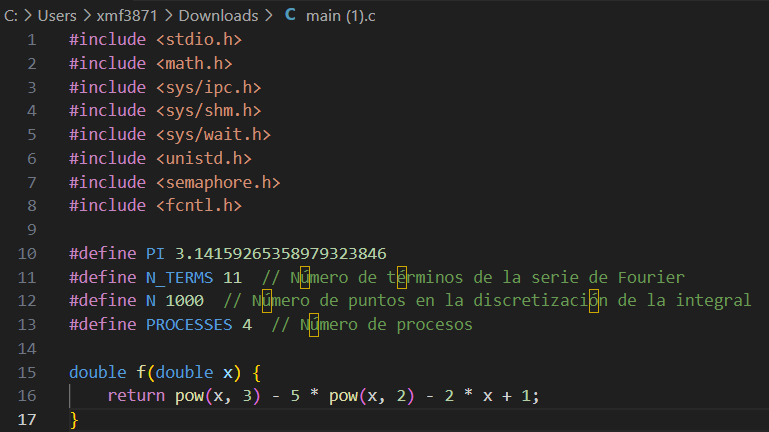
\includegraphics[width=5.55729in,height=3.12944in]{media/image18.png}
		\caption{Código}
	\end{figure}
	
	\item La función \emph{calculate coefficients} se encarga de calcular los coeficientes de la serie de Fourier para un rango de términos n específico. Utiliza una técnica de sincronización con semáforos para garantizar que cada proceso realice sus cálculos de manera ordenada.
	
	\begin{figure}[H]
		\centering
		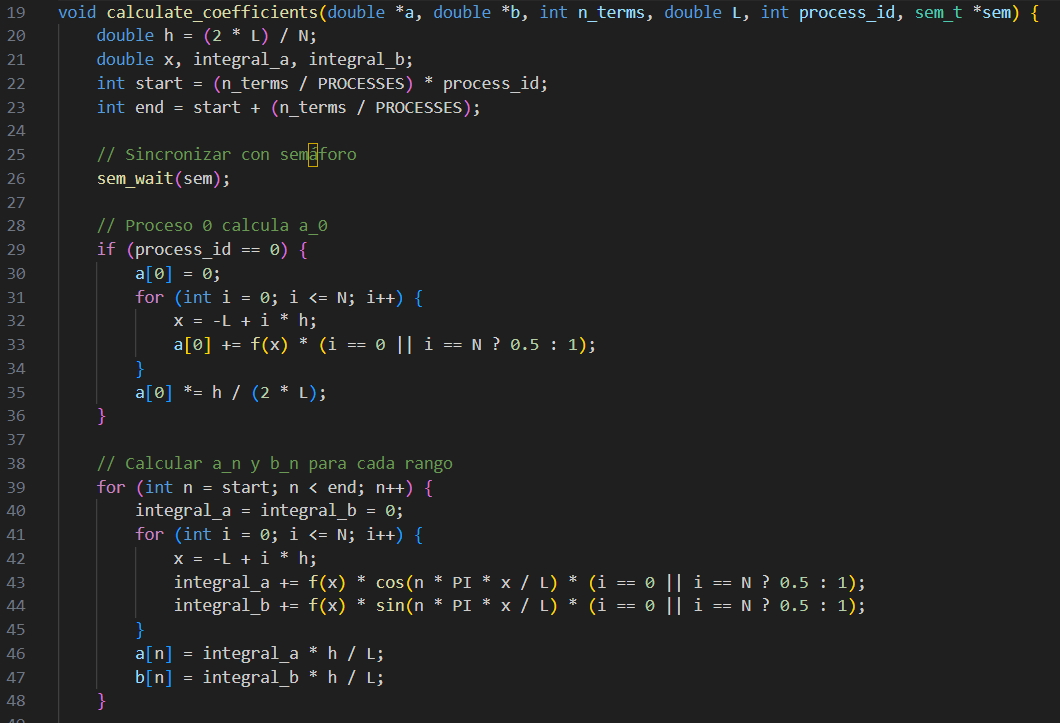
\includegraphics[width=5.64741in,height=3.85562in]{media/image39.png}
		\caption{Función calculate coefficients}
	\end{figure}
	
	\item La función \emph{fourier\_approximation} calcula la aproximación de la función original utilizando los coeficientes de la serie de Fourier.
	
	\begin{figure}[H]
		\centering
		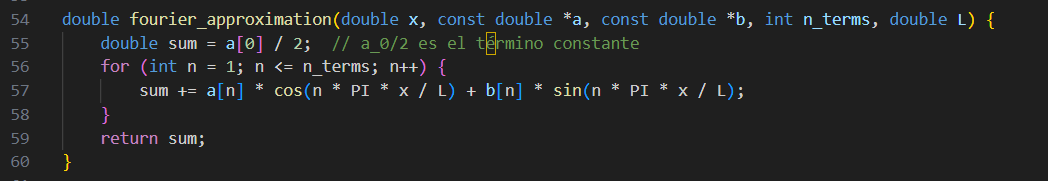
\includegraphics[width=6.26772in,height=1.08333in]{media/image11.png}
		\caption{Función fourier approximation}
	\end{figure}
	
	\item La función \emph{export\_to\_csv} exporta los resultados a un archivo CSV que contiene los valores de x, la función original y la aproximación de la serie de Fourier y\_fourier.
	
	\begin{figure}[H]
		\centering
		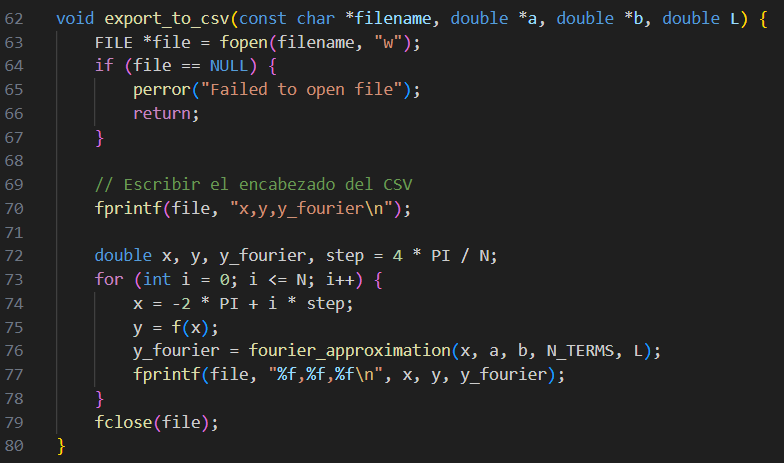
\includegraphics[width=5.02604in,height=2.61756in]{media/image50.png}
		\caption{Función export\_to\_csv}
	\end{figure}
	
	\item En la función main, se crea un segmento de memoria compartida para almacenar los coeficientes a y b, se crea un semáforo para la sincronización entre procesos y se generan varios procesos hijos para calcular los coeficientes de la serie de Fourier en paralelo. Después de que todos los procesos hayan terminado de calcular los coeficientes, se exportan los resultados a un archivo CSV y se liberan los recursos utilizados.
	
	\begin{figure}[H]
		\centering
		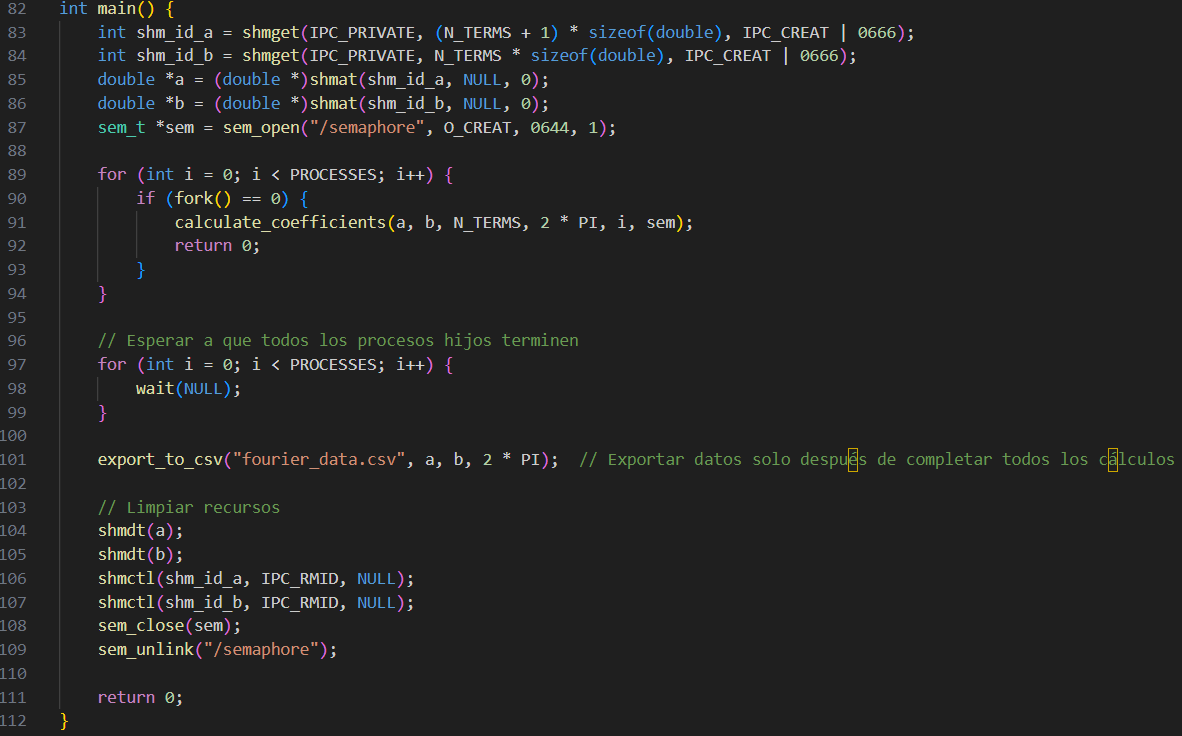
\includegraphics[width=6.26772in,height=3.90278in]{media/image7.png}
		\caption{Función main}
	\end{figure}
	
\end{enumerate}

\subsection{Ejecución del código}

\begin{enumerate} 
	\def\labelenumi{\arabic{enumi}.} 
	\item Ejecución de código en linux
	
	\begin{figure}[H]
		\centering
		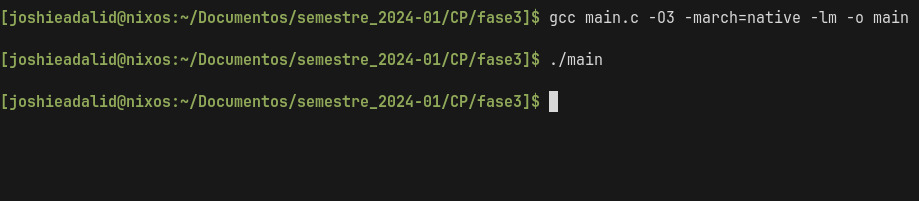
\includegraphics[width=6.26772in,height=1.375in]{media/image29.png}
		\caption{Ejecución en Linux}
	\end{figure}
	
	\item Visualización del archivo generado. Para cada x, su evaluación en la función a aproximar, y su aproximación de la serie de Fourier.
	
	\begin{figure}[H]
		\centering
		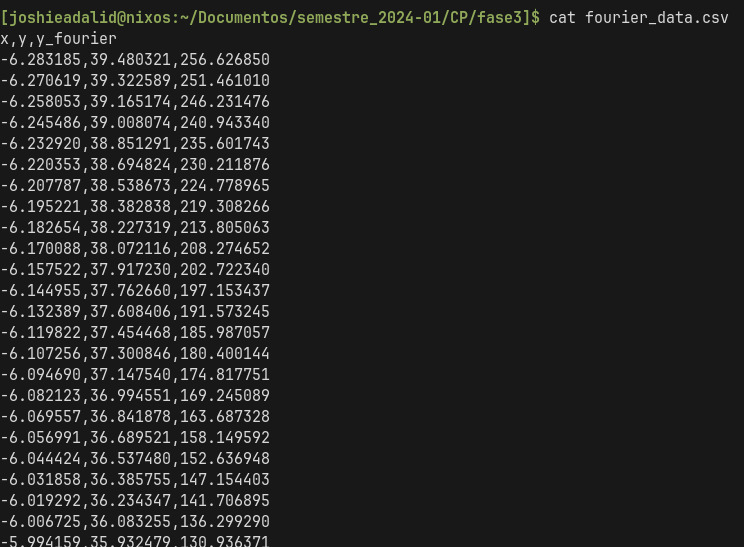
\includegraphics[width=5.16146in,height=3.79822in]{media/image37.png}
		\caption{Aproximación para la serie de Fourier}
	\end{figure}
	
	\begin{figure}[H]
		\centering
		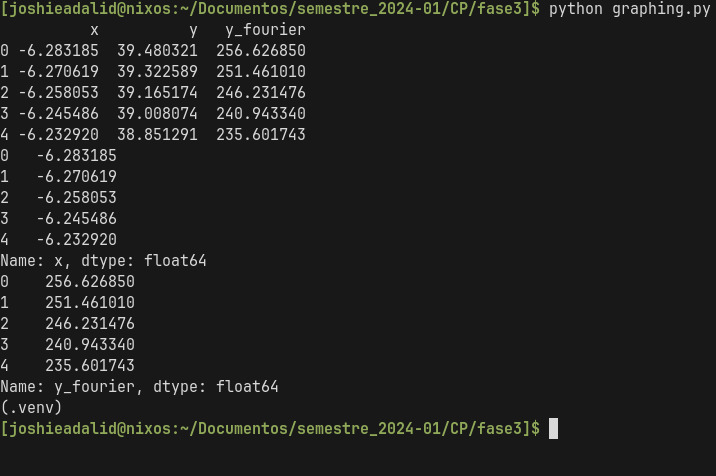
\includegraphics[width=5.16146in,height=3.42309in]{media/image25.png}
		\caption{Aproximación para la serie de Fourier}
	\end{figure}
	
	\item Gráfica generada
	
	\begin{figure}[H]
		\centering
		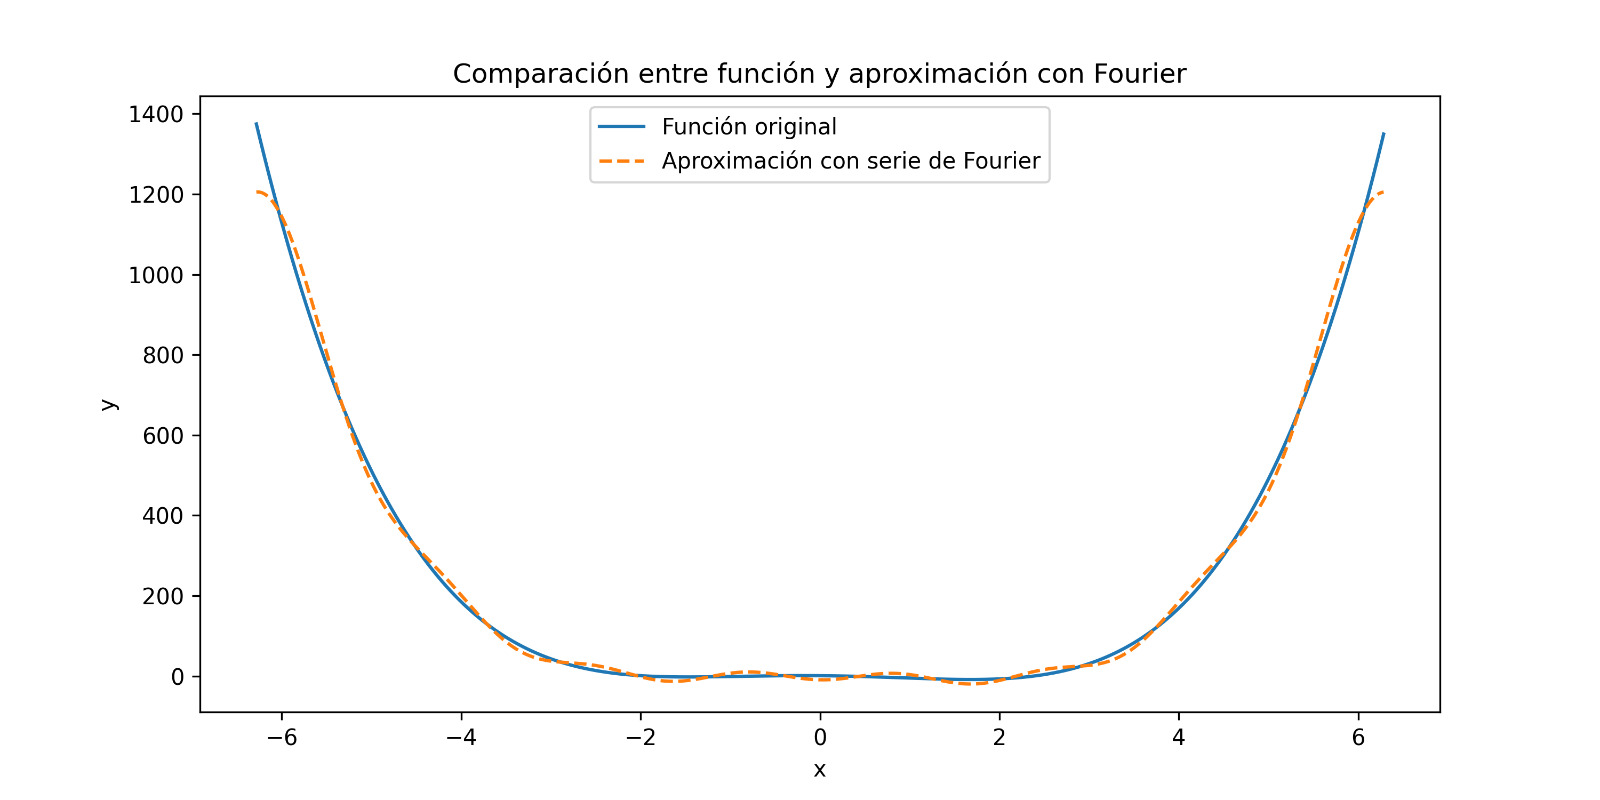
\includegraphics[width=6.26772in,height=3.13889in]{media/image12.png}
		\caption{Gráfica original y aproximación de Fourier en C}
	\end{figure}
	
\end{enumerate}

\subsection{Implementación de código con hilos}

En este apartado se mostrará y explicará el código implementado ahora con hilos en lugar de memoria compartida y semáforos.

\begin{enumerate} 
	\def\labelenumi{\arabic{enumi}.} 
	\item En primer lugar, se incluyen las bibliotecas necesarias para utilizar las funciones básicas y las funciones de hilos como se muestran en la imagen 13, así como definir unas constantes que nos ayudarán a ejecutar el programa con hilos.
	
	\begin{figure}[H]
		\centering
		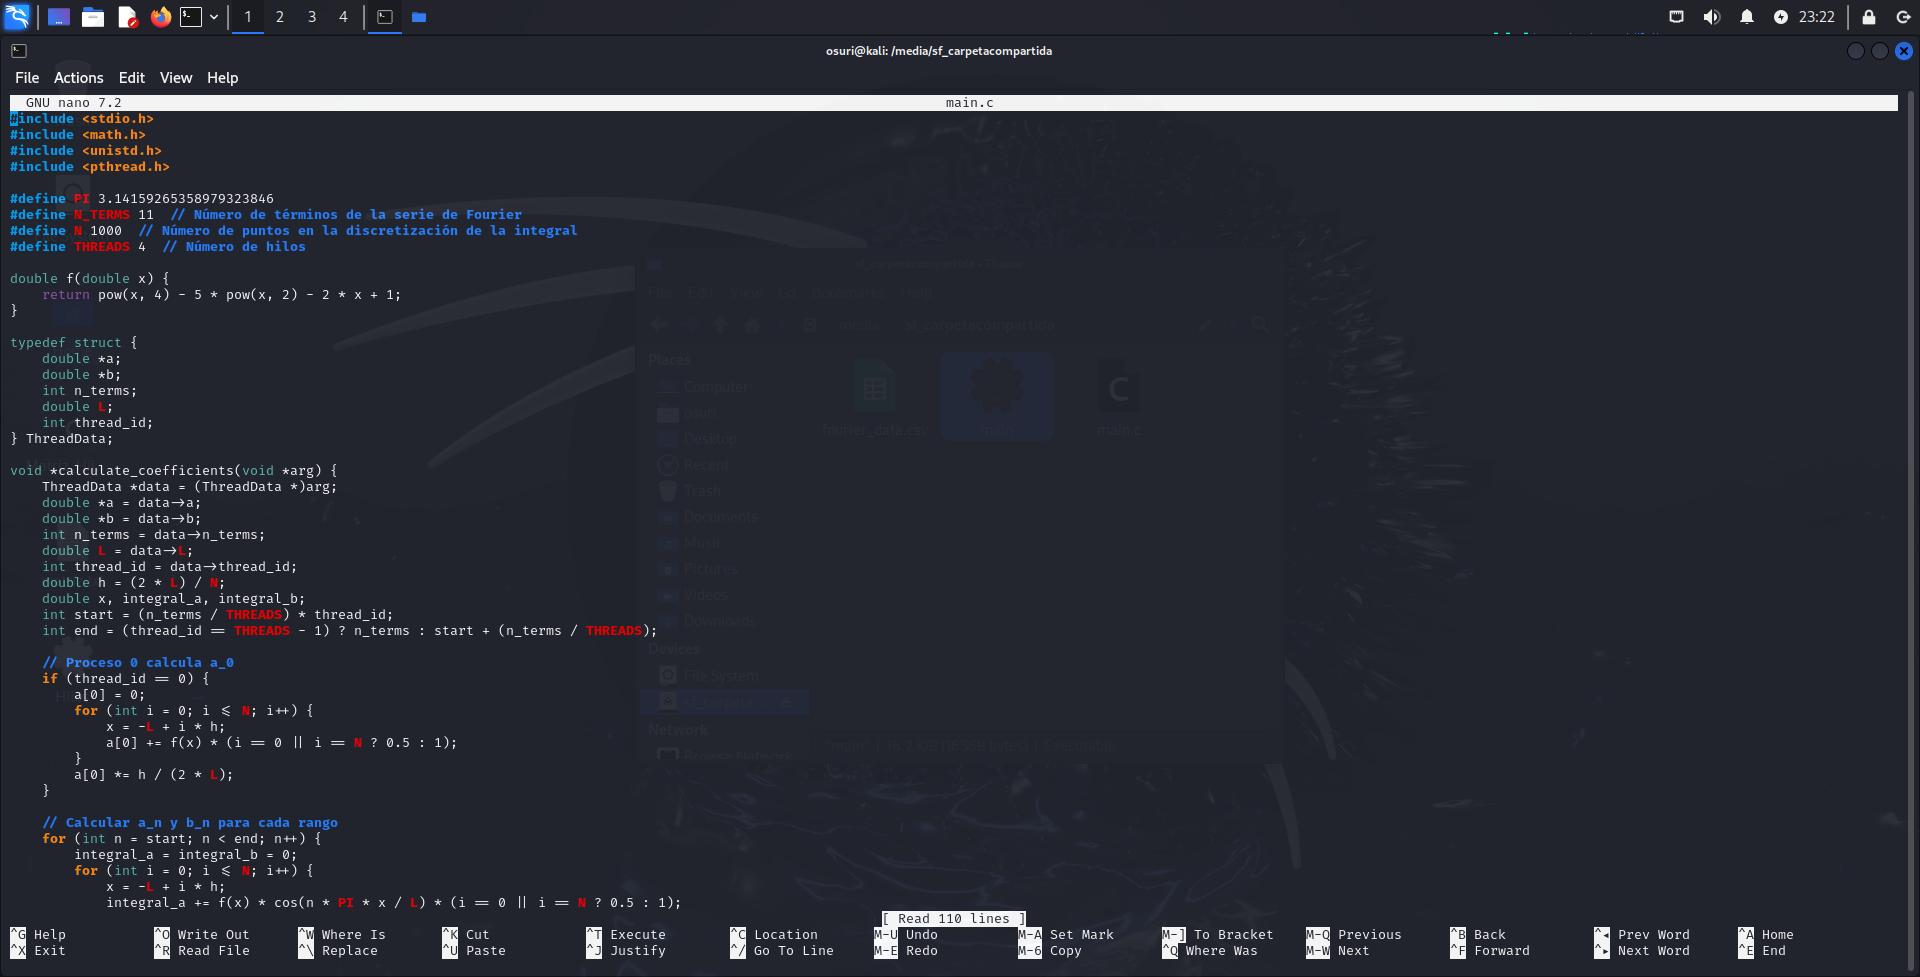
\includegraphics[width=4.53385in,height=1.24967in]{media/image4.png}
		\caption{Código 1. Fuente: Autoría propia}
	\end{figure}
	
	\item En la imagen 14 se define la estructura básica de la serie original y se crea la estructura de un hilo para que tenga los datos de la ecuación de la serie, así como los valores que debe de calcular, para almacenar múltiples tipos de datos y no entre en conflicto.
	
	\begin{figure}[H]
		\centering
		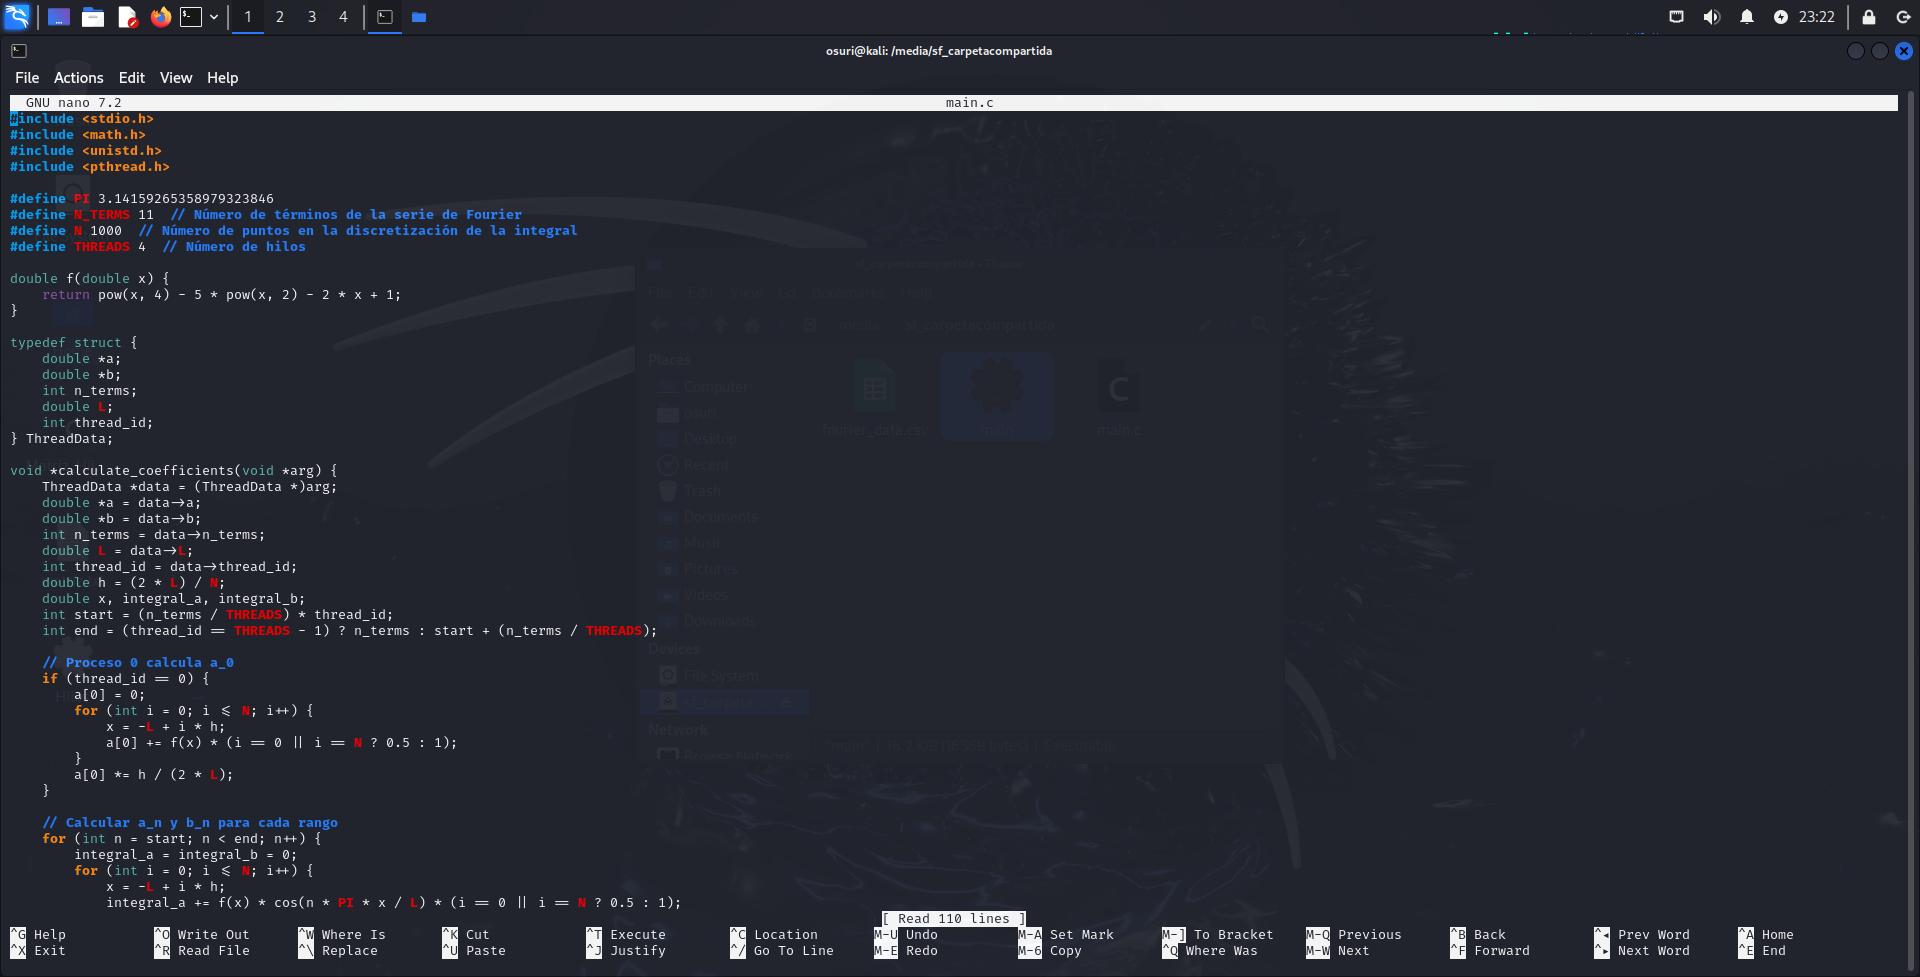
\includegraphics[width=3.15in,height=1.54172in]{media/image4.png}
		\caption{Código 2. Fuente: Autoría propia}
	\end{figure}
	
	\item En la imagen 15, se define una función para resolver la serie de Fourier por medio de hilos, se divide la información para que pueda ser ejecutada miles de veces, y se crean los hilos separados para resolver los cálculos. Se pone separado el cálculo de a0 porque sólo se calcula una vez, mientras que an y bn deben ser calculados tantas veces como "n" existan.
	
	\begin{figure}[H]
		\centering
		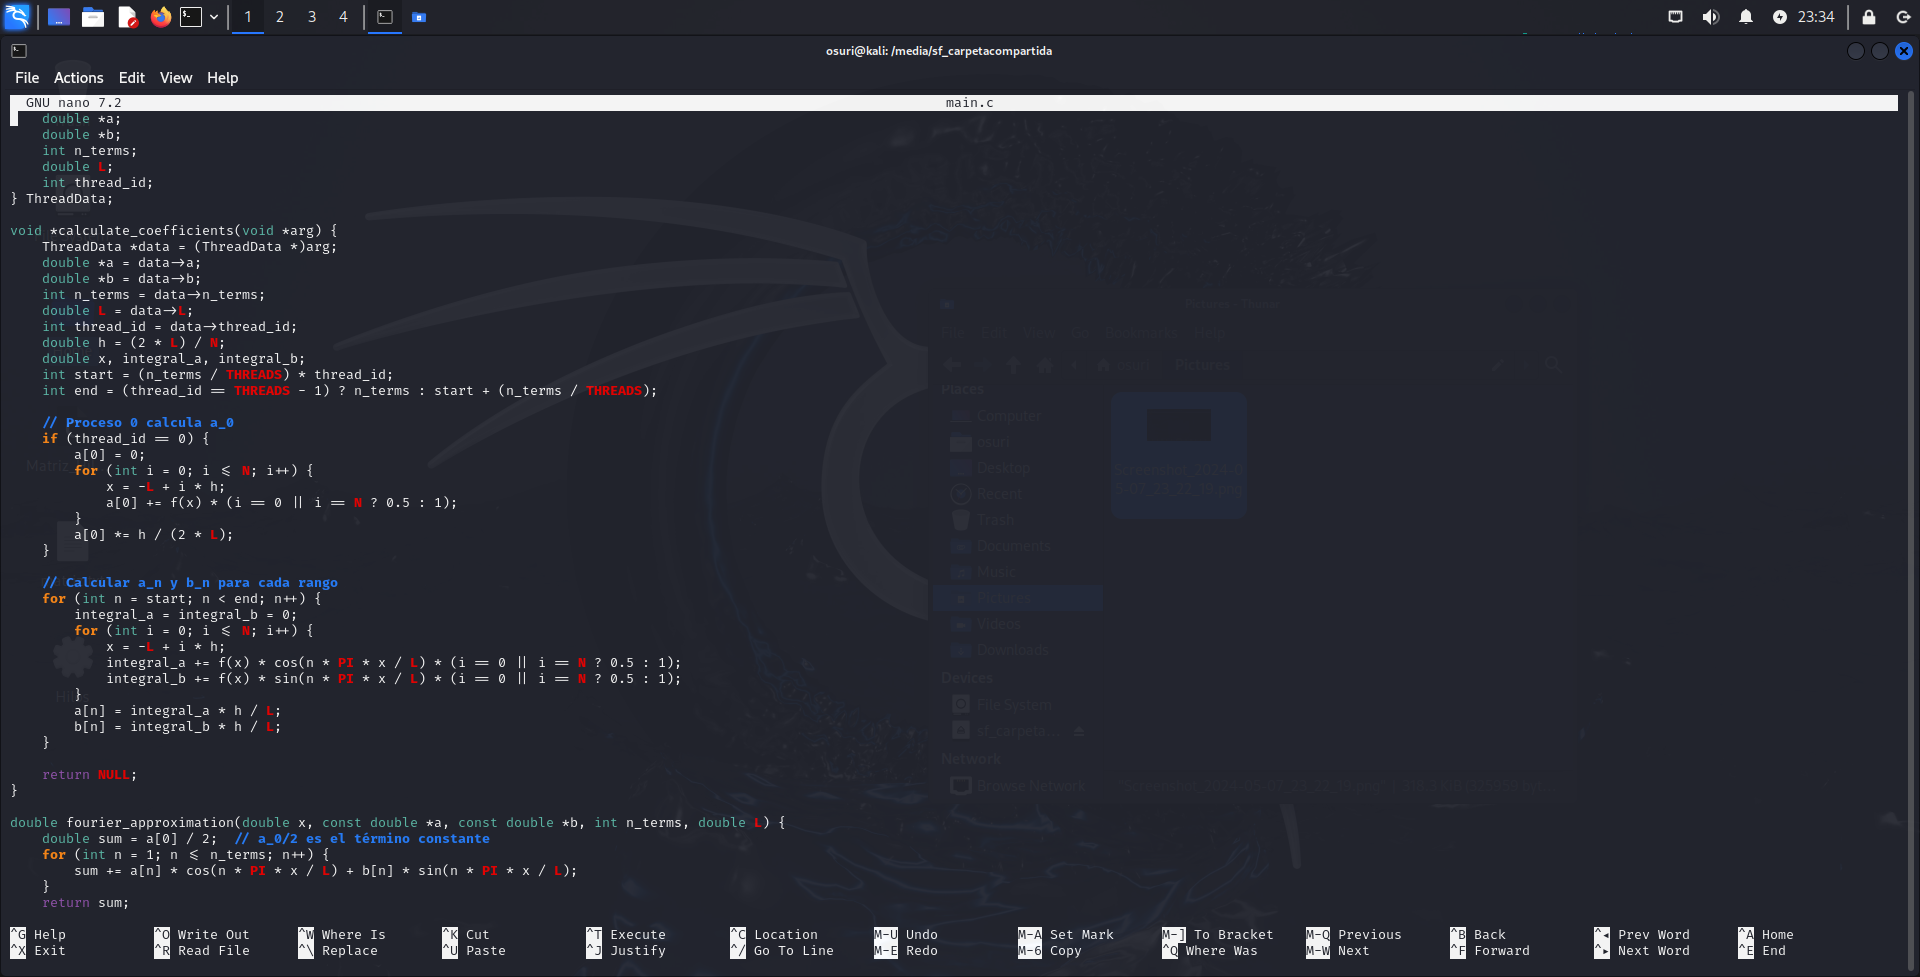
\includegraphics[width=3.00416in,height=2.52623in]{media/image17.png}
		\caption{Código 3. Fuente: Autoría propia}
	\end{figure}
	
	\item En la imagen 16 se crea una función de aproximación con la serie original para comparar los valores.
	
	\begin{figure}[H]
		\centering
		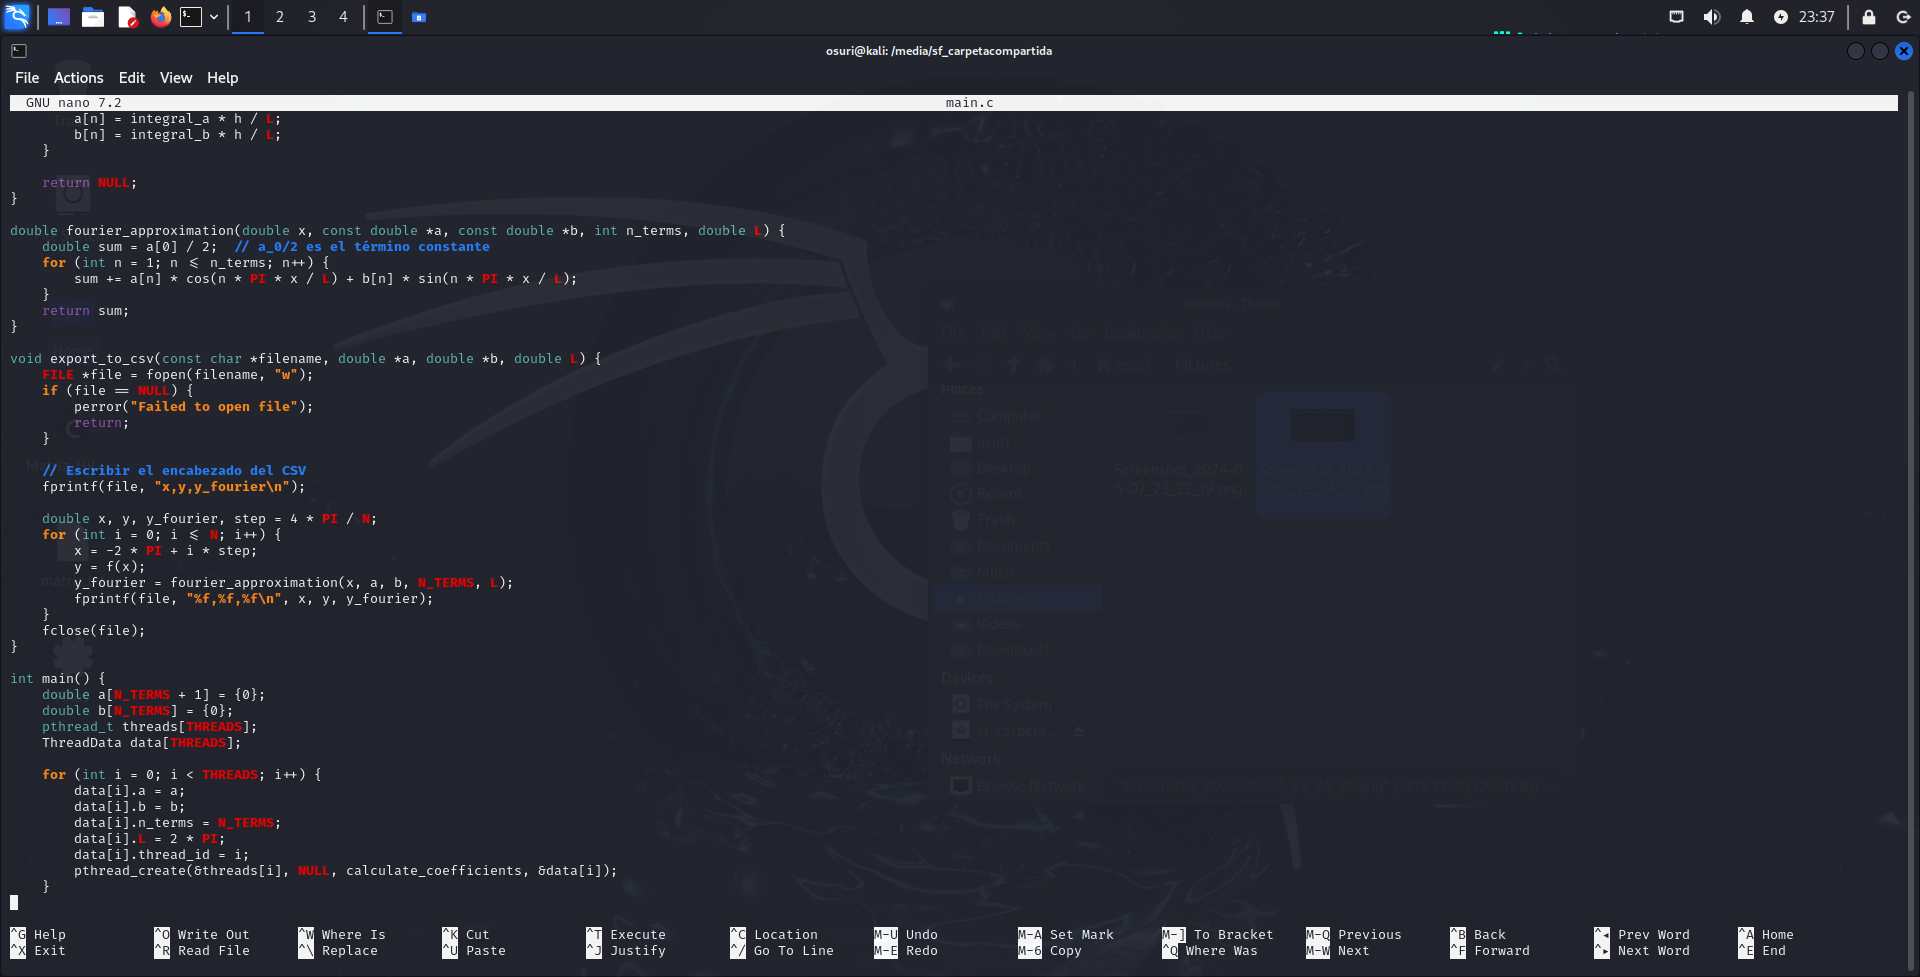
\includegraphics[width=4.31145in,height=0.71292in]{media/image27.png}
		\caption{Código 4. Fuente: Autoría propia}
	\end{figure}
	
	\item En la imagen 17, se crea la función para exportar los cálculos exitosos a un archivo CSV para poder guardarlos y consultarlos.
	
	\begin{figure}[H]
		\centering
		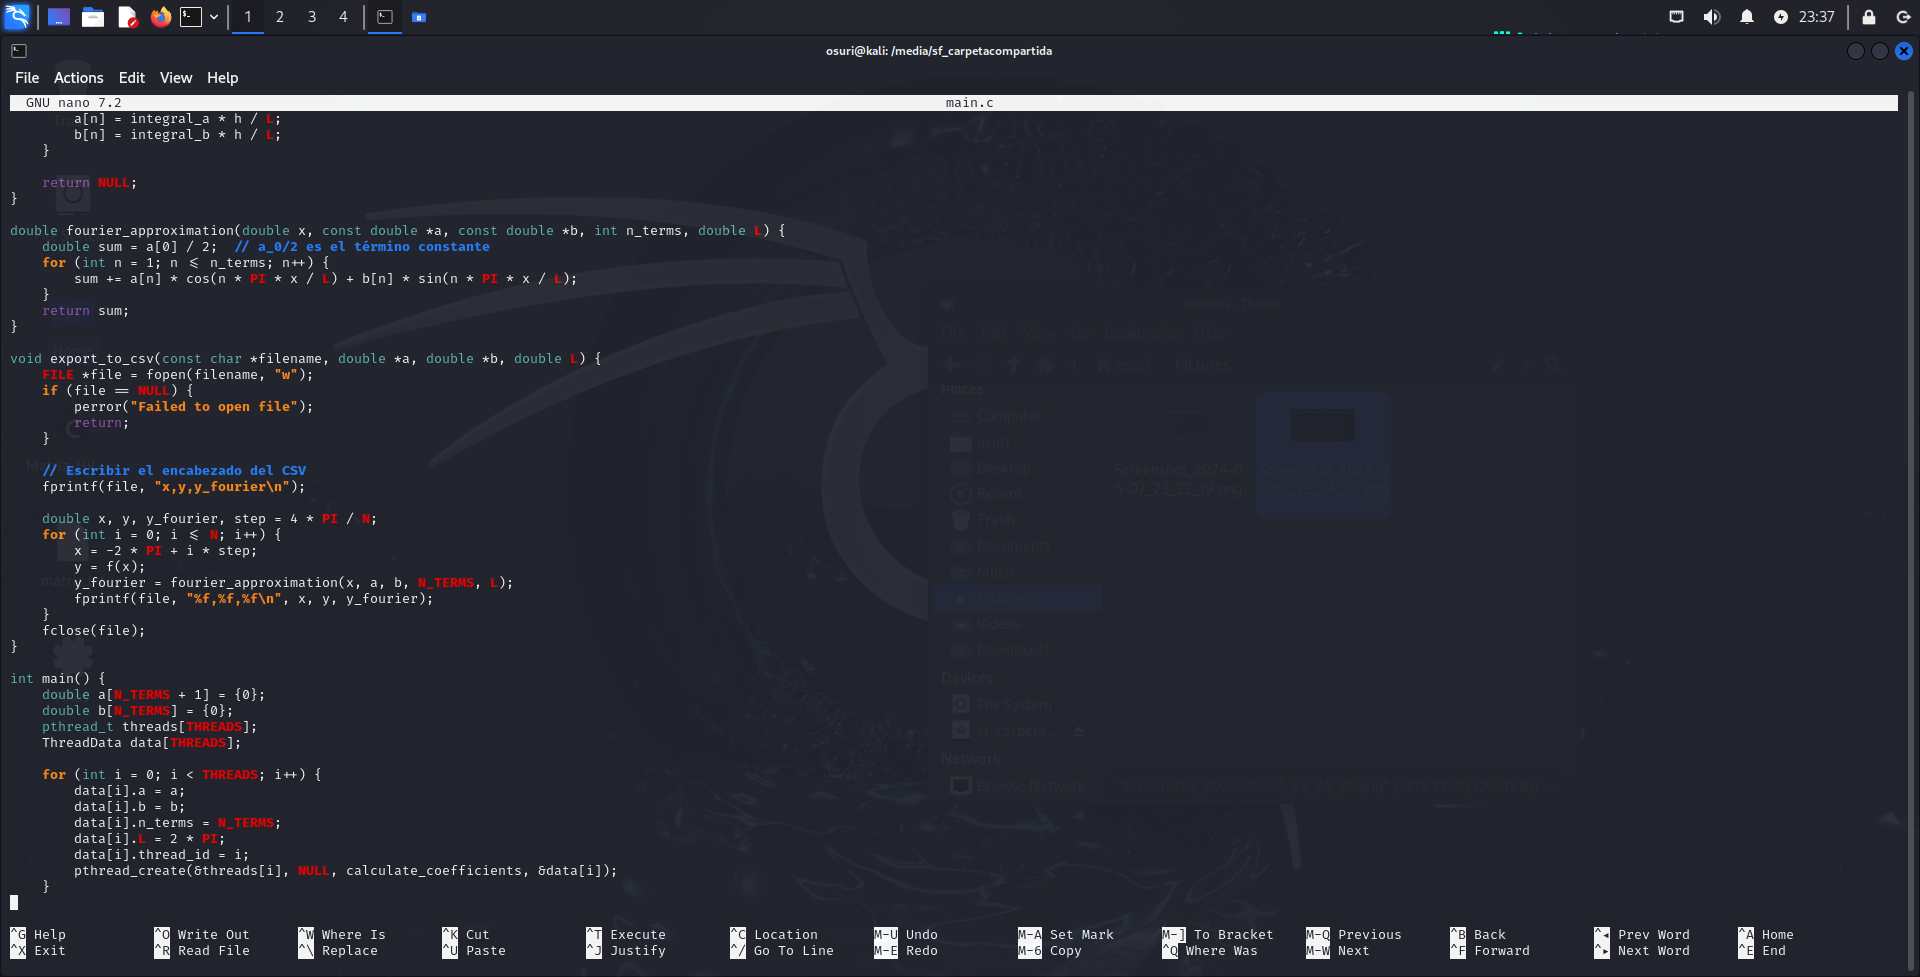
\includegraphics[width=4.19531in,height=2.2036in]{media/image27.png}
		\caption{Código 5. Fuente: Autoría propia}
	\end{figure}
	
	\item En la imagen 18, se puede observar el programa main, donde se ejecuta el proceso principal, se crean los hilos de acuerdo a la cantidad de veces que se ejecutará la secuencia, en este caso 1000, se utilizará la estructura del hilo definida con anterioridad para ejecutar los hilos, y finalmente se utilizará la función para exportar a CSV para guardar los datos.
	
	\begin{figure}[H]
		\centering
		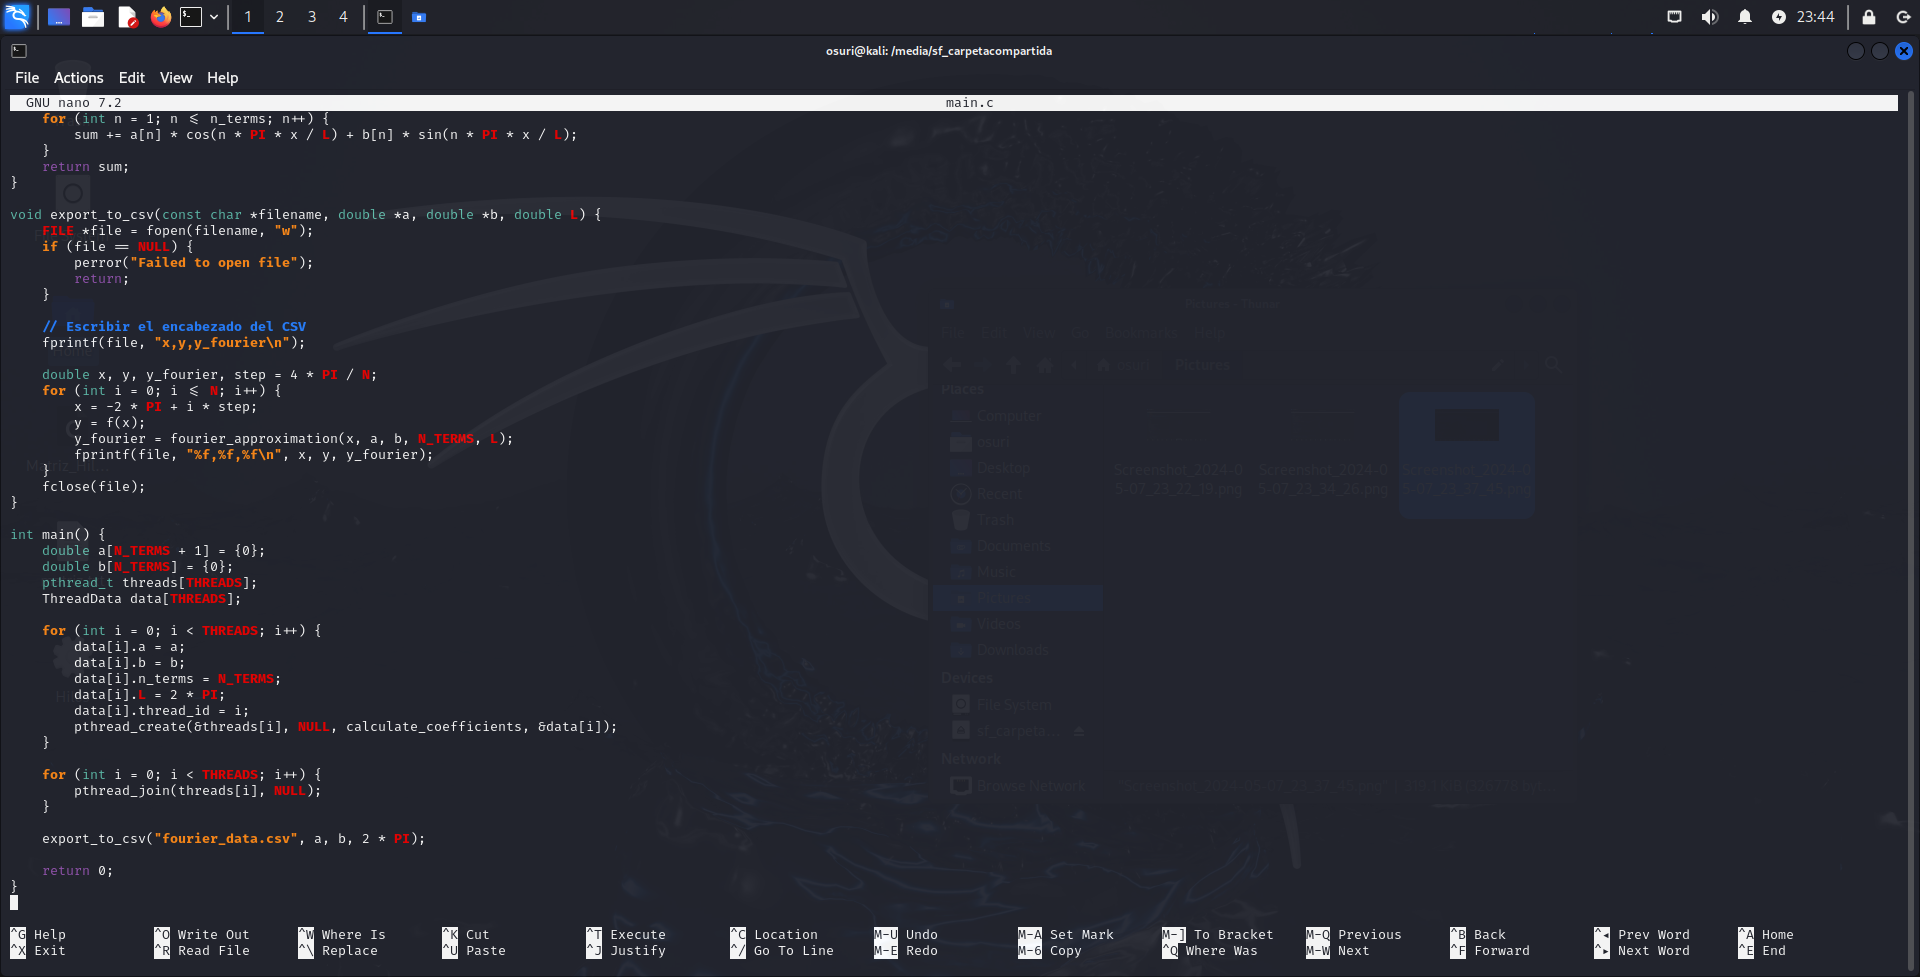
\includegraphics[width=3.82031in,height=2.4068in]{media/image5.png}
		\caption{Código 6. Fuente: Autoría propia}
	\end{figure}
	
\end{enumerate}

\subsection{Ejecución del código con hilos}

\begin{enumerate} 
	\def\labelenumi{\arabic{enumi}.} 
	\item Compilación y ejecución (ver imagen 19).
	
	\begin{figure}[H]
		\centering
		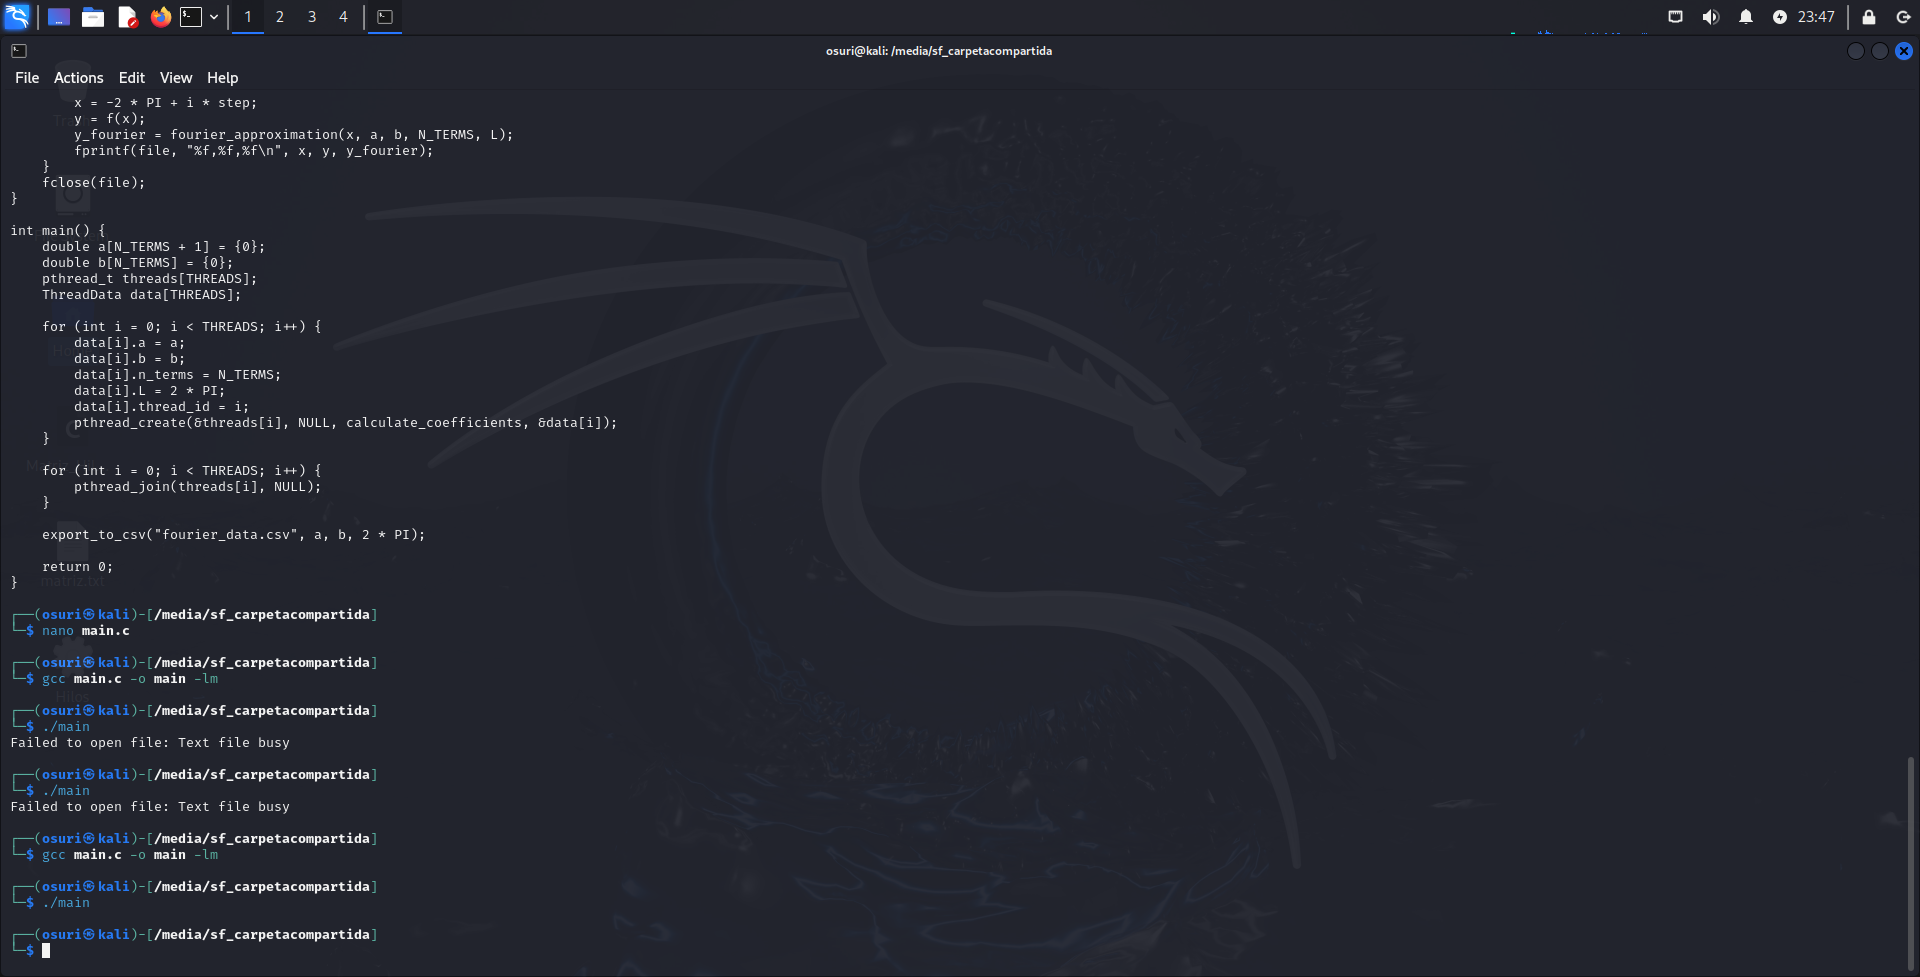
\includegraphics[width=3.46875in,height=0.8384in]{media/image36.png}
		\caption{Compilación y ejecución. Fuente: Autoría propia}
	\end{figure}
	
	\item Visualización menor de datos, solo se utilizan ciertos datos para no saturar el documento (ver imagen 20).
	
	\begin{figure}[H]
		\centering
		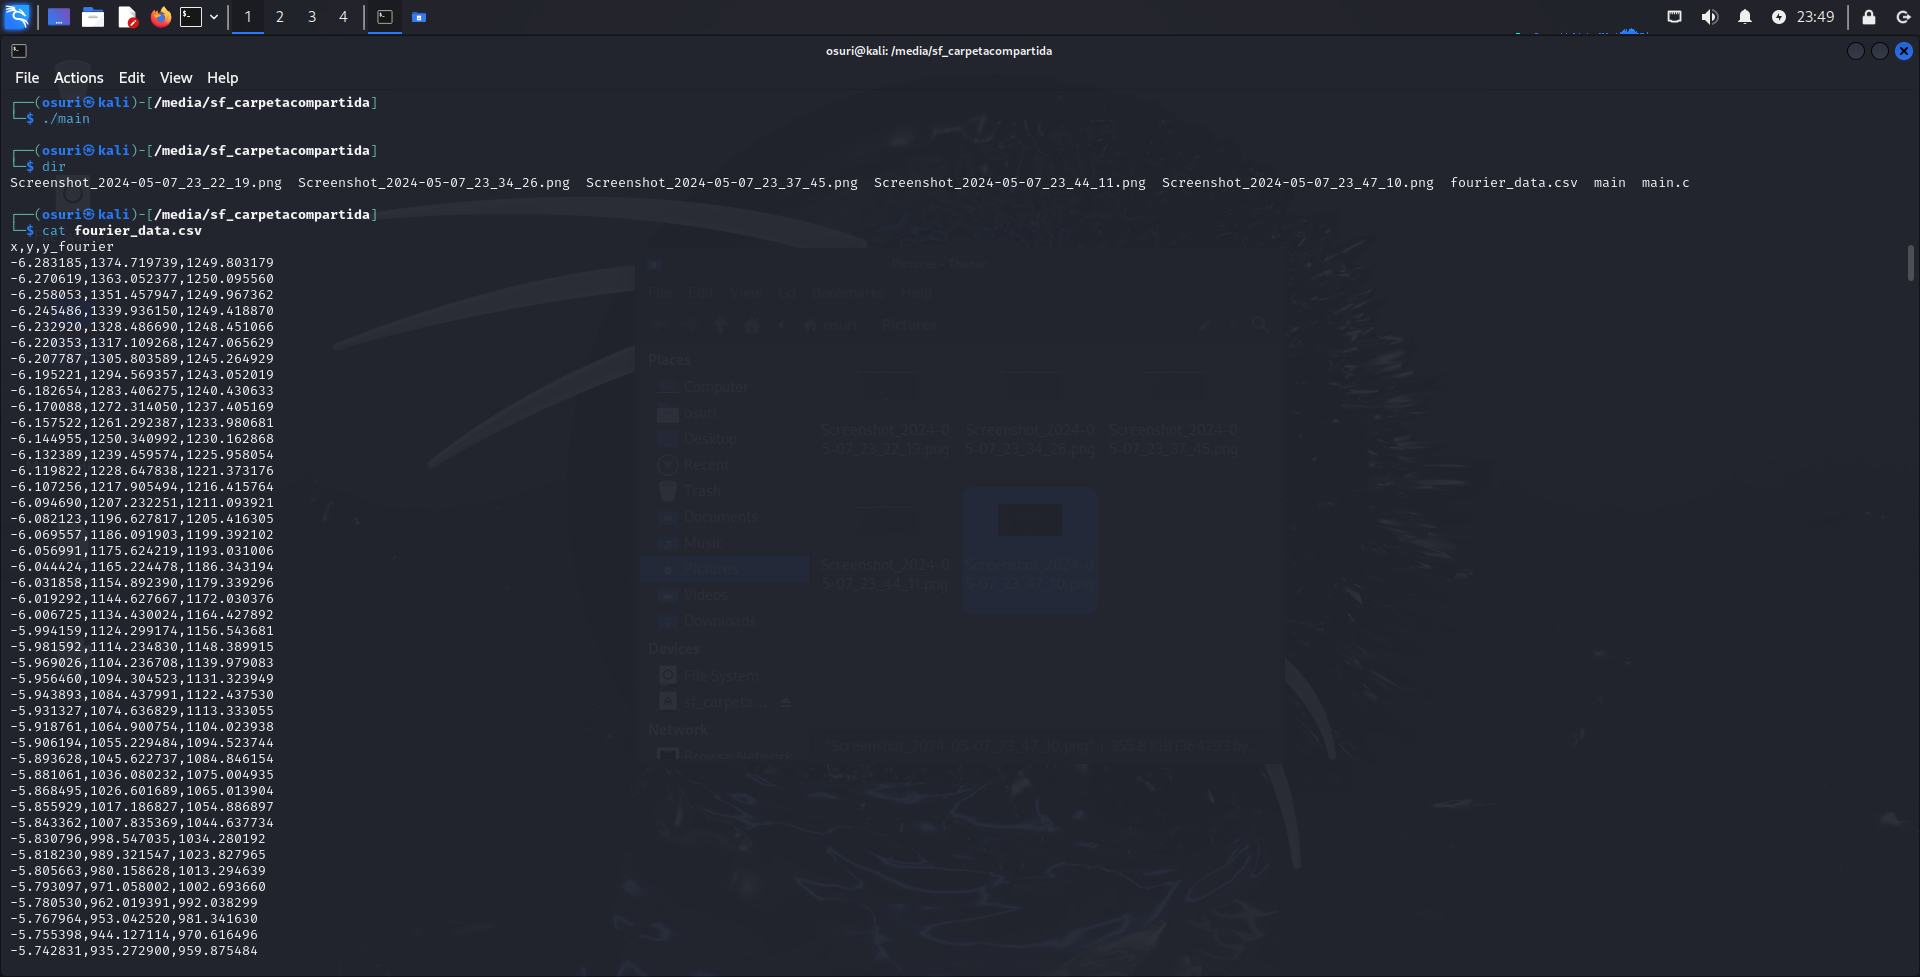
\includegraphics[width=2.29583in,height=4.29598in]{media/image35.png}
		\caption{Datos de archivo CSV. Fuente: Autoría propia}
	\end{figure}
	
	\item Gráfica generada por este conjunto de datos (ver figura 5)
	
	\begin{figure}[H]
		\centering
		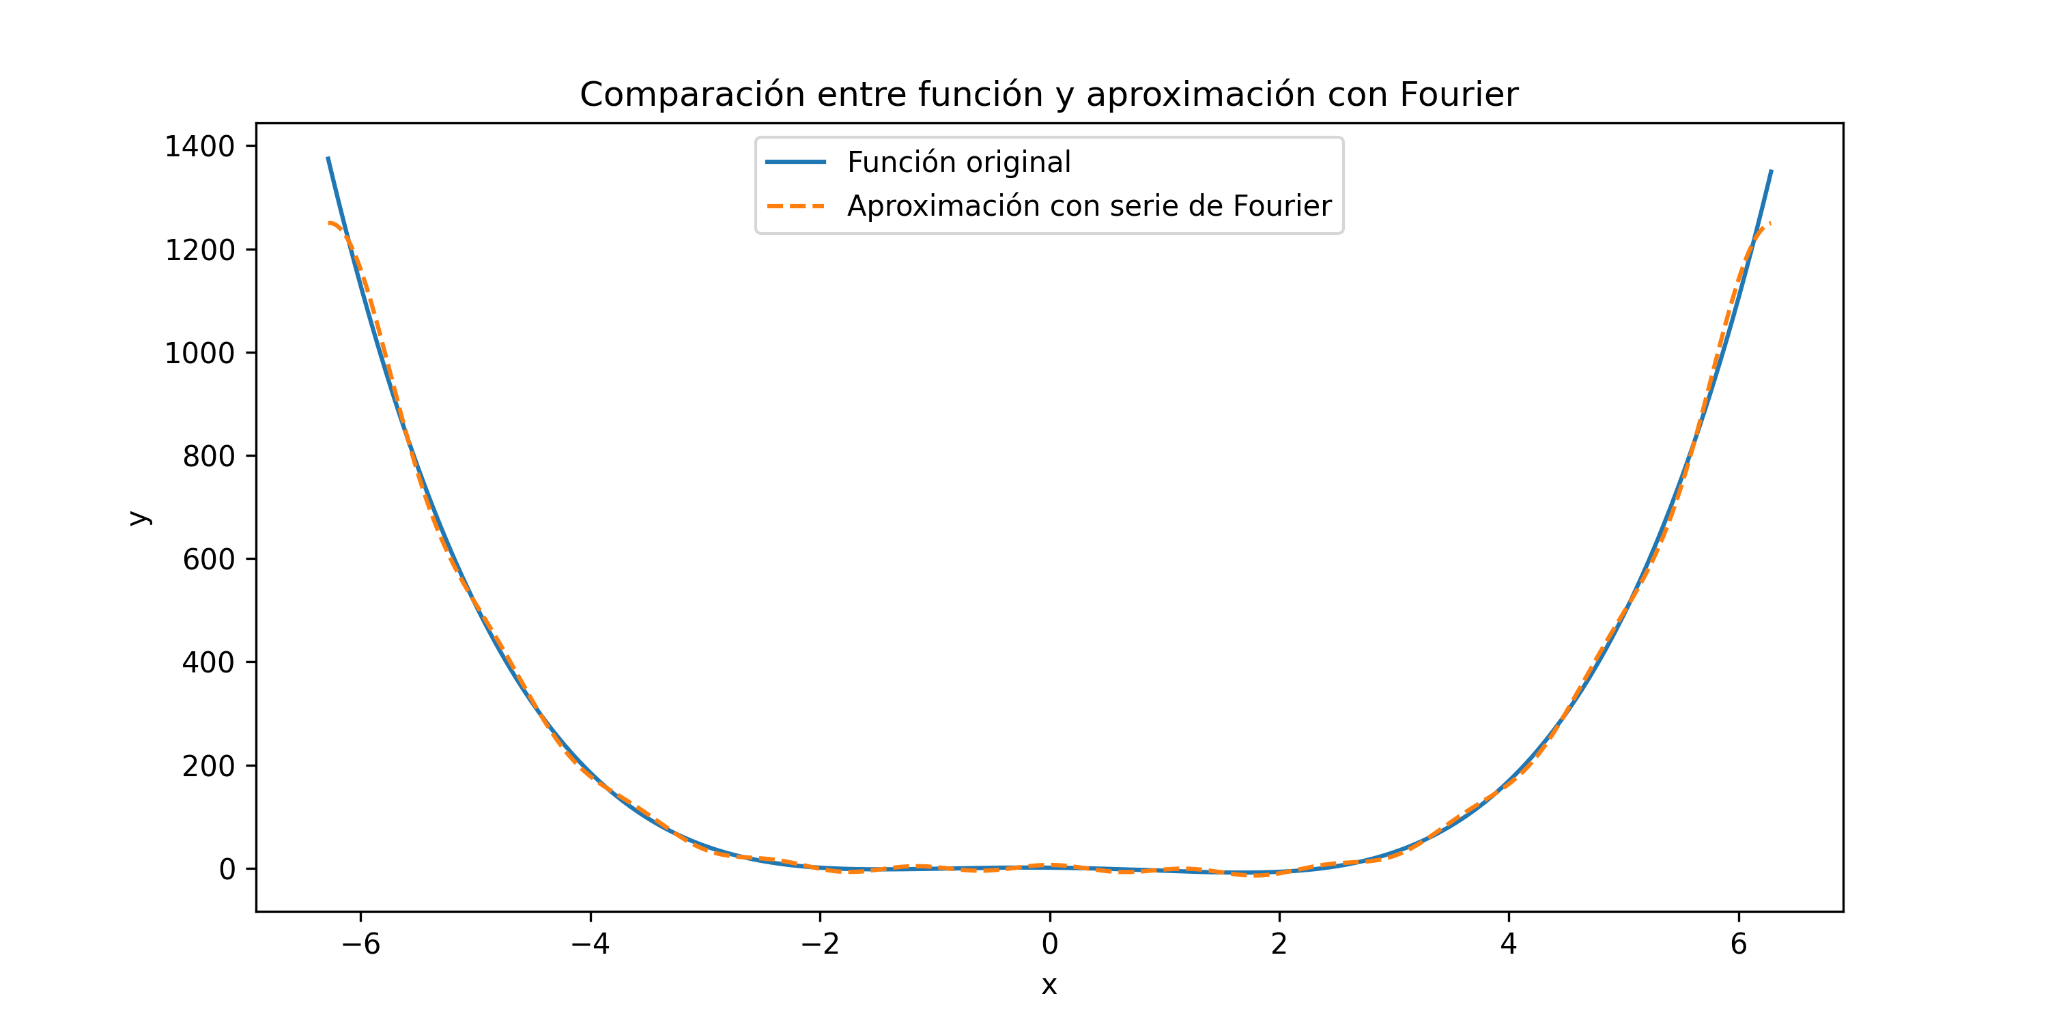
\includegraphics[width=6.26772in,height=3.13889in]{media/image30.png}
		\caption{Gráfica generada. Fuente: Autoría propia}
	\end{figure}
	
\end{enumerate}

\subsection{Ejecución del código con MPI}
\begin{figure}[H]
	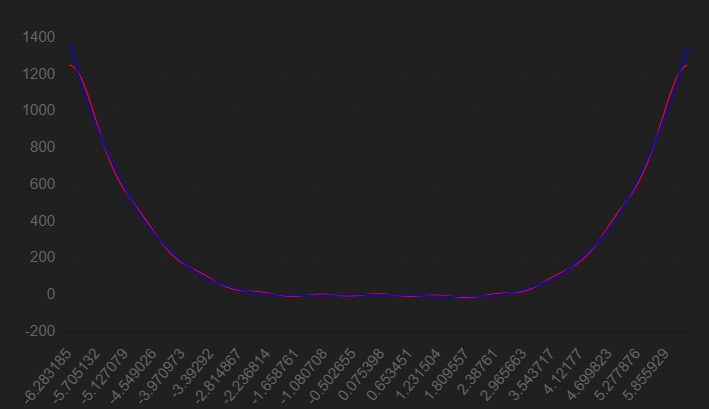
\includegraphics[width=0.8\textwidth]{media/mpi_grafica.jpeg}
	\caption{Comparación de la función original contra la aproximación de la serie de Fourier, calculado con la tecnología de MPI}
\end{figure}

\begin{figure}[H]
	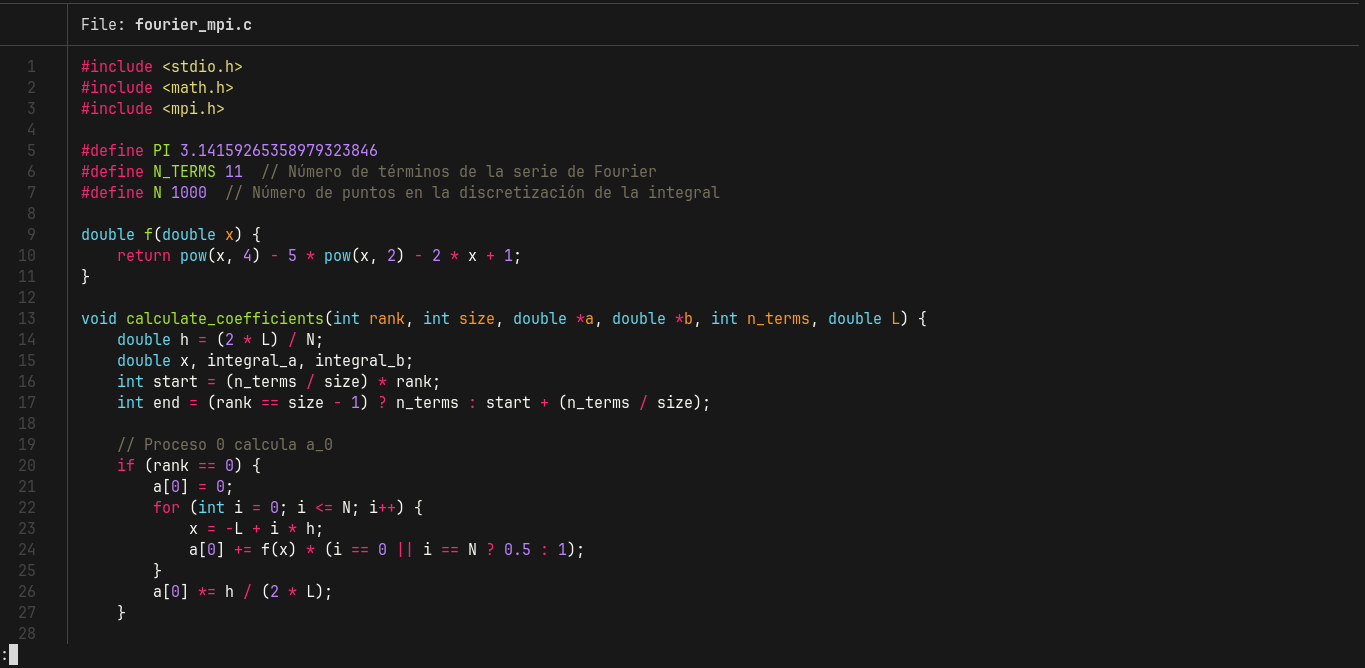
\includegraphics[width=0.8\textwidth]{media/mpi_codigo_1.png}
	\caption{Fragmento del código fuente en C para MPI. Parte 1 de 4.}
\end{figure}
\begin{figure}[H]
	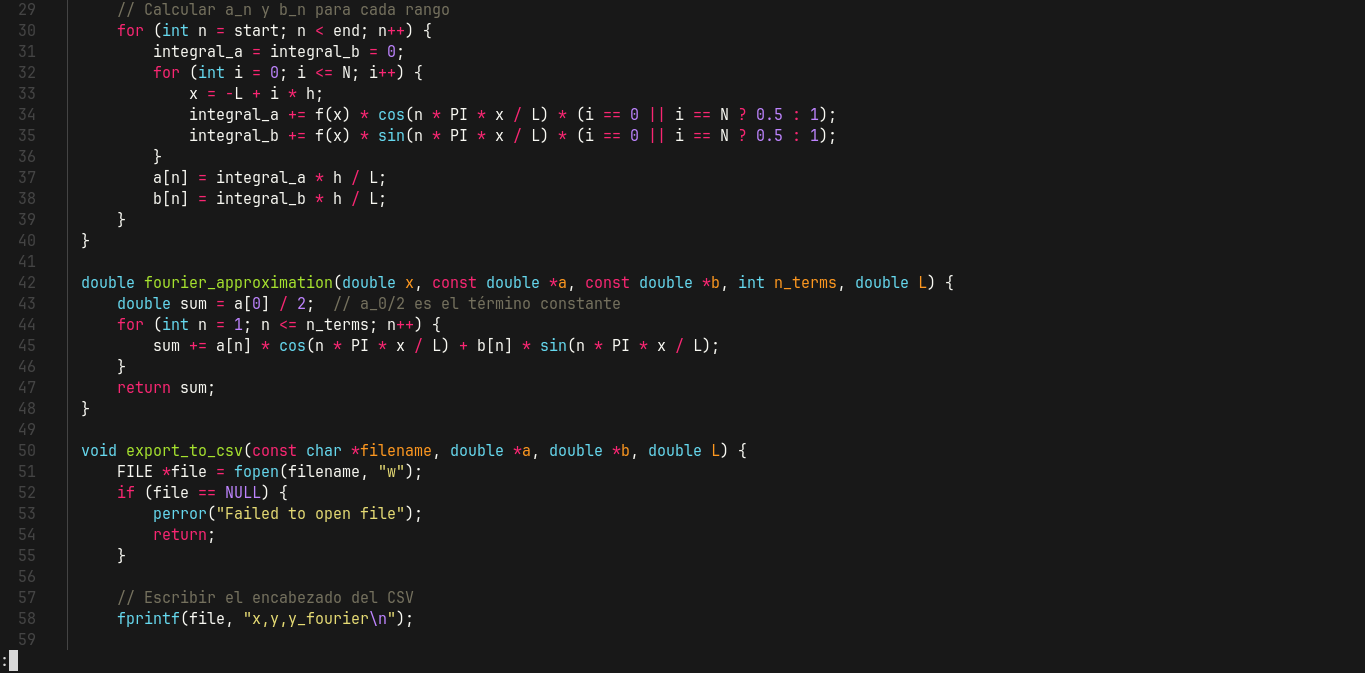
\includegraphics[width=0.8\textwidth]{media/mpi_codigo_2.png}
	\caption{Fragmento del código fuente en C para MPI. Parte 2 de 4.}
\end{figure}
\begin{figure}[H]
	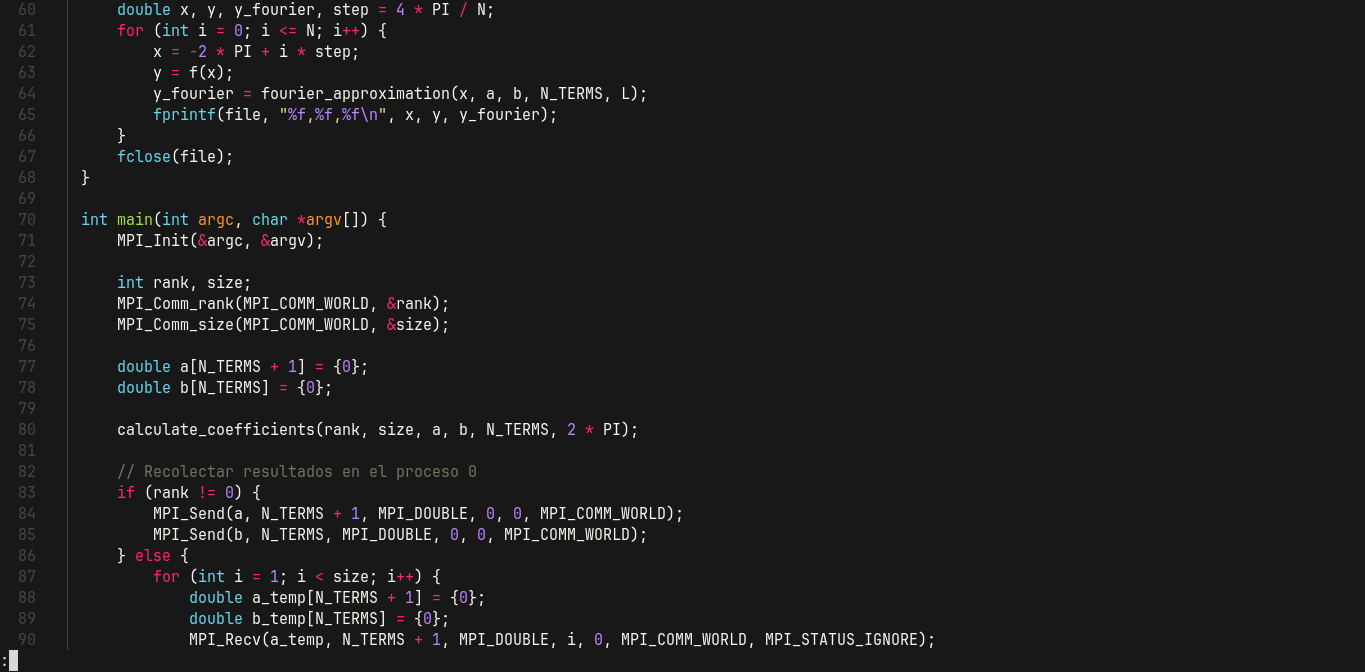
\includegraphics[width=0.8\textwidth]{media/mpi_codigo_3.png}
	\caption{Fragmento del código fuente en C para MPI. Parte 3 de 4.}
\end{figure}
\begin{figure}[H]
	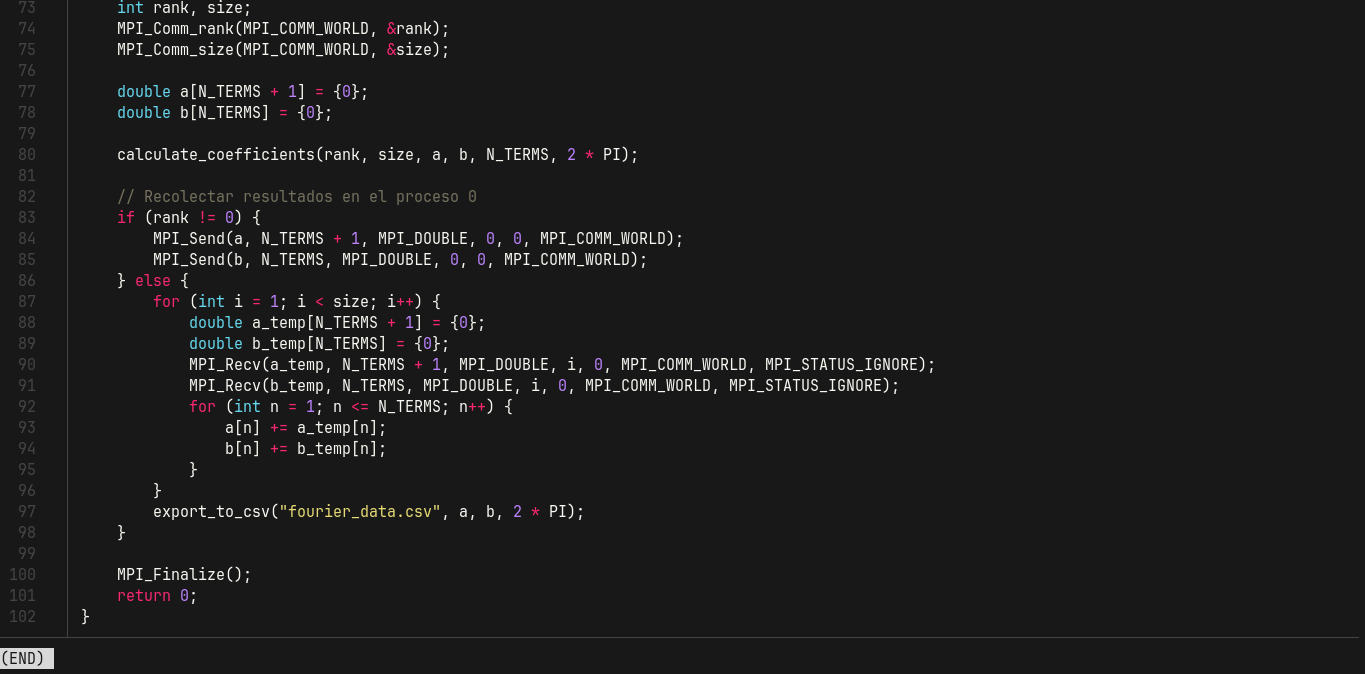
\includegraphics[width=0.8\textwidth]{media/mpi_codigo_4.png}
	\caption{Fragmento del código fuente en C para MPI. Parte 4 de 4.}
\end{figure}